\documentclass[aspectratio=169]{beamer}
\usepackage{fancyvrb}
\usepackage{framed}
\usepackage{caption}
\usepackage{qrcode}
\usetheme{CambridgeUS}

\usepackage{listings}
\usepackage{xcolor}
\usepackage{tikz}
\usetikzlibrary{shapes.geometric, arrows}
\tikzstyle{process} = [rectangle, minimum width=3cm, text centered, draw=black, fill=orange!30]
\tikzstyle{decision} = [rectangle, minimum width=3cm, text centered, draw=black, fill=green!30]
\tikzstyle{code} = [rectangle, minimum width=3cm, text centered, draw=black, fill=yellow!20]
\tikzstyle{arrow} = [thick,->,>=stealth]
\tikzstyle{arrow2} = [thick, dashed, ->,>=stealth]
\tikzstyle{arrow3} = [thick, ->, draw=blue]

\title[hevm]{
hevm, a flexible symbolic execution framework to verify EVM bytecode}
\author[dxo, Soos, Paraskevopoulou]{dxo, \emph{Mate Soos}, Zoe Paraskevopoulou}
\institute[Argot]{\large Argot Collective (\url{https://argot.org})}
\date{7th of March 2025, BSA Conference, Switzerland}


\begin{document}
\begin{frame}
    \titlepage 
\end{frame}

%\begin{frame}{A bit about myself}
%\begin{itemize}
%\item PhD from INRIA Grenoble, France, wrote CryptoMiniSat, a SAT solver with the theory of Gauss-Jordan elimination
%\item Worked in IT Security industry for 10+ years
%\item Research at Kuldeep Meel's group for the past 5 years, mostly on counting and sampling
%\item Working at Ethereum Foundation for the past 2 years
%\end{itemize}
%\bigskip
%
%A lot of what I did were rewrite systems: preprocessors, inprocessors, etc. hevm is in large part, a rewrite system
%\end{frame}

% Outline frame
\begin{frame}{Outline}
    \tableofcontents
\end{frame}

\section{What is Symbolic Execution}

% \begin{frame}{A Quick Recap of Ethereum}
% Ethereum is the second largest cryptocurrency in terms of value. Ethereum has:
% \begin{itemize}
% \item Contracts with \textbf{code and storage}, unlike e.g. Bitcoin
% \item Stack-based VM, the EVM. Most popular executor of EVM: \textbf{geth}
% \item ACID execution semantics, like a \textbf{database}
% \item Proof-of-stake as its \textbf{consensus layer} -- ordering transactions
% \end{itemize}

% Downsides:
% \begin{itemize}
% \item Code and data are not clearly separated ("EOF" will solve)
% \item JUMP destinations are known, but dynamic jumps are possible
% \item All EVM instructions operate on 256b values
% \end{itemize}

% \end{frame}

\begin{frame}[fragile=singleslide]{Symbolic Execution vs Fuzzing}
Say your code is:

\begin{Verbatim}[frame=single, framerule=0.2mm, framesep=2mm,fontsize=\small]
function tricky(uint a, uint b) public pure {
	// solution: a = 10000983843024
	//           b = 9877982748934
	
	if (a * 2 + b == 29879950434982 &&
	    b / 2 == 4938991374467) {
		assert(false); // bad things happen
	}
}
\end{Verbatim}

Fuzzing never finds this edge-case. Symbolic execution always finds it.
\bigskip 

\textbf{In general, fuzzing is faster, but is incomplete. Symbolic execution is slower but complete.}

\end{frame}



\begin{frame}[fragile=singleslide]{Symbolic Execution: straight line program}

Most execution works by running instructions concretely:
\begin{verbatim}
---             ax: 1   , bx: 2
mov %bx %ax     ax: 2   , bx: 2
add %ax $4      ax: 6   , bx: 2
\end{verbatim}
\bigskip

Symbolic execution, with symbolic state:
\begin{verbatim}
---             ax: v1  , bx: v2
mov %bx %ax     ax: v2  , bx: v2
add %ax $4      ax: v2+4, bx: v2
\end{verbatim}
\end{frame}

\begin{frame}[fragile=singleslide]{Symbolic Execution -- branching}
\begin{minipage}[t]{0.45\textwidth}
Concrete execution:
\begin{Verbatim}[fontsize=\small]
-----------     ax: 1    bx: 1
cmp %ax %bx     ax: 1    bx: 1
je .if_true     
; false
add %ax $4
jmp short .end
.if_true:
add %ax $5      ax: 6    bx: 1
.end:
\end{Verbatim}
\end{minipage}%
\begin{minipage}[t]{0.45\textwidth}
Symbolic execution, with symbolic state:
\begin{Verbatim}[fontsize=\small]
-----------     ax: v1   bx: v2
cmp %ax %bx     
je .if_true     
; false
add %ax $4      ax: v1+4 bx: v2
jmp short .end
.if_true:
add %ax $5      ax: v1+5 bx: v2
.end:
\end{Verbatim}
\begin{Verbatim}[fontsize=\small]
-**- v1==v2 ->  ax: v1+5 bx: v2
-**- v1!=v2 ->  ax: v1+4 bx: v2
\end{Verbatim}
\end{minipage}
\bigskip

For symbolic execution, we end up having to follow two executions. This can become exponential.
\end{frame}


\begin{frame}{Related Work}

Symbolic execution is used in two major ways. One is to \textbf{validate static code analysis} results, the other is \textbf{pure symbolic execution}. The first approach is followed by Oyente, sCompile, Mythril, etc. These are typically incomplete, and false positives are allowed.

\bigskip

Purely symbolic execution-based systems:
\begin{itemize}
\item \textbf{halmos}: Written in python, with its own IR and internal rewrite engine
\item \textbf{Certora Prover}: Based on backwards exploration and weakest precondition computation
\item \textbf{KEVM}: K-framework based, allows to ``break out'' into K to prove lemmas
\item \textbf{EthBMC}: Bounded model checking-based exploration of contracts
\end{itemize}
\end{frame}


\section{Overview of hevm}
\begin{frame}{Overview of hevm}
\begin{itemize}
\item Started $\approx7$ years ago as part of dapptools, but is now a standalone tool
\item Implements EVM semantics for concrete and symbolic execution
\item Examines \emph{all}\footnote{loops/recursion is an issue, we have a loop/depth limit} execution paths from the starting state
\item Finds the set of requirements to reach all failing paths
\item Runs external SMT solver(s) to find input to reach them
\item Displays call needed to trigger:
\begin{itemize}
    \item the fault: \texttt{hevm test}
    \item the discrepancy: \texttt{hevm equivalence}
\end{itemize}
\end{itemize}
\end{frame}


%\begin{frame}[fragile=singleslide]{Symbolic Execution: example}
%Say your code looks like this:
%\begin{Verbatim}[frame=single, framerule=0.2mm, framesep=2mm,fontsize=\small]
%function overflow(uint a) public pure {
%	uint b;
%	unchecked { b = a + 1;}
%	assert(b > a);
%}
%\end{Verbatim}
%
%
%hevm can find the case where $a=0xffffff\ldots$ to trigger the assert due to roll-around. hevm gives you the \textbf{exact call to reproduce the bug}. This way of using hevm can find a \emph{known-bad state}.
%
%\end{frame}



%\begin{frame}[fragile=singleslide]{Symbolic Execution: Invariant Checking}
%You can describe \textbf{invariants} of your contract and write them as functions Then assert these functions every time the invariant must hold.
%\begin{Verbatim}[frame=single, framerule=0.2mm, framesep=2mm,fontsize=\small]
%function my_invariant() private pure returns inv {
%	inv = ...calculate invariant...
%}
%	
%function transfer(uint a) public pure {
%	require(my_invariant());
%	... your function code here ....
%	assert(my_invariant());
%}
%\end{Verbatim}
%
%Here, instead of a known-bad state, we validate that we are always in state that matches our expectations.
%\end{frame}	

\begin{frame}{hevm: Symbolic Execution for Counterexample Generation}
\centering
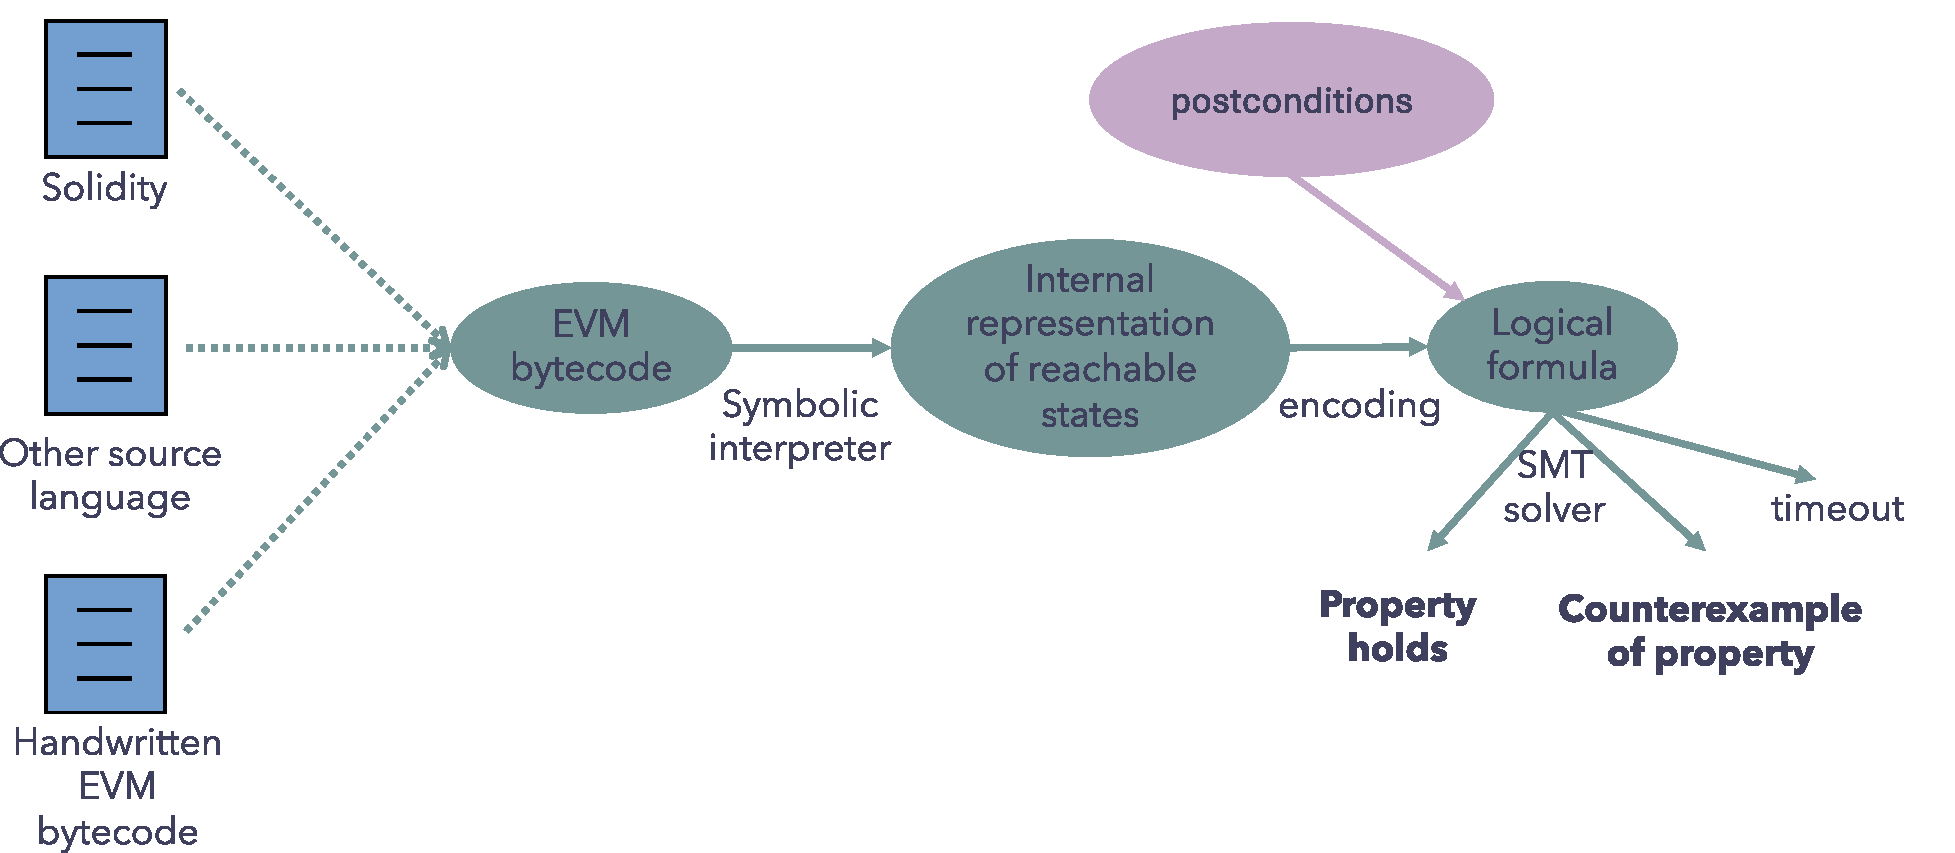
\includegraphics[scale=0.45]{pipeline}
\end{frame}

\begin{frame}{hevm: Symbolic Execution for Equivalence Checking}
\centering
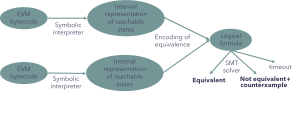
\includegraphics[scale=0.45]{equivalence-pipeline}
\end{frame}
%
%
%\begin{frame}[fragile=singleslide]{hevm: Symbolic Execution for Equivalence Checking}
%You can ask hevm to check whether two implementations are equivalent
%\bigskip
%\\
%
%\begin{minipage}[b]{0.45\textwidth}
%\begin{Verbatim}[frame=single, framerule=0.2mm, framesep=2mm,fontsize=\small]
%function (...) public returns x {
%  x = /known good computation/
%      /uses lots of gas/
%}
%    \end{Verbatim}
%  \end{minipage}
%  \begin{minipage}[b]{0.45\textwidth}
%  \begin{Verbatim}[frame=single, framerule=0.2mm, framesep=2mm,fontsize=\small]
%function (...) public returns x {
%  x = /complicated computation/
%      /uses less gas/
%}
%\end{Verbatim}
%\end{minipage}
%
%hevm can give the exact \textbf{call to trigger the discrepancy} between the two functions. This way, you can safely improve the gas performance of your code.
%\end{frame}

\begin{frame}{hevm's Symbolic Executor}
hevm's symbolic executor is very powerful:
\begin{itemize}
\item \textbf{Operates on bytecode} so runs everything deployed to the chain
\item Understands \textbf{all of EVM}: stack, call frames, memory, storage, calldata
\item Can run on \textbf{any point in blockchain history} via RPC to an archive node
\item Pull all required contracts from the chain via RPC to a full node
\item Overapproximates unknown code
\item Fuzzed against concrete execution (geth) for correctness
\end{itemize}
\bigskip

Limitations:
\begin{itemize}
\item Cannot deal with \textbf{symbolic gas} other than ignoring it
\item \textbf{Symbolic offset/size memcopy} is not implemented, but is often unneeded
\item \textbf{Loops and recursion} are explored only to a fixed depth
\end{itemize}
\end{frame}

\begin{frame}{hevm internals}
\centering
\includegraphics[scale=0.6]{hevm-overview}
\end{frame}


\begin{frame}[fragile=singleslide]{Intermediate Representation}
\small

Through the symbolic execution engine we create an expression that captures all end-states. We then take each end-state out and filter it for things we are looking for, e.g. assertion failures. Let's take the example:

\begin{Verbatim}[frame=single, framerule=0.2mm,framesep=2mm,fontsize=\small]
function overflow(uint a) public pure {
	uint b;
	unchecked { b = a + 1;}
	assert(b > a);
}
\end{Verbatim}

The expression to generate a counterexamle for this could look like:

\begin{Verbatim}[frame=single, framerule=0.2mm, framesep=2mm,fontsize=\small]
PLEq (Add (Var "a") (Lit 1)) (Var "a")
\end{Verbatim}

Notice: we use less-or-equal, because we want a \textbf{counterexample}
\end{frame}

%\begin{frame}[fragile]{Intermediate Representation}
%\begin{tikzpicture}[node distance=2cm]
%\centering
%\tiny
%%ITE node

%%the source code
%\node (program) [code]
%{\begin{lstlisting}[numbers=none]
%contract MyContract {
%  mapping(uint => uint) items;
%  function test(uint val1) public {
%    require(val1 > 10);
%    unchecked {
%      items[4] = val1+1;
%      assert(items[4] > 10); } } }
%\end{lstlisting}};

%\node (dec1) [decision, right of=program, xshift=6.5cm]
%%\node[draw, align=left] at (6,7)
%{\begin{lstlisting}[numbers=none]
%(ITE (IsZero TxValue)) ...
%\end{lstlisting}};

%% left of that:
%%\node[draw, align=left] at (0,6)
%\node (pro1) [process, below of=program, yshift=0.3cm]
%{\begin{lstlisting}[numbers=none]
%(Failure Error: Revert)
%  Assertions:
%    (PEq (IsZero TxValue) 0 )
%    (PLT (BufLength (AbstractBuf "txdata")) 18446744073709551616 )
%\end{lstlisting}};

%% ITE node after:
%%\node[draw, align=left] at (6,6)
%\node (dec2) [decision, below of=dec1, yshift=0.5cm]
%{\begin{lstlisting}[numbers=none]
%ITE (LT 10 (Var "arg1")) ...
%\end{lstlisting}};

%% left of that:
%%\node[draw, align=left] at (0,4)
%\node (pro2) [process, below of=pro1, yshift=0.5cm]
%{\begin{lstlisting}[numbers=none]
%(Failure Error: Revert [..])
%  Assertions:
%    (PEq (LT 10 (Var "arg1")) 0 )
%    (PEq TxValue 0 )
%    (PLT (BufLength (AbstractBuf "txdata")) 18446744073709551616 )
%\end{lstlisting}};

%% ITE node after:
%%\node[draw, align=left] at (6,4)
%\node (dec3) [decision, below of=dec2, yshift=0.5cm]
%{\begin{lstlisting}[numbers=none]
%ITE (LT (Add 1 (Var "arg1")) 10)...
%\end{lstlisting}};

%%left of that:
%%\node[draw] at (0,2)
%\node (pro3) [process, below of=pro2, yshift=0.5cm]
%{\begin{lstlisting}[numbers=none]
%(Failure Error: Revert [...])
%  Assertions:
%    ....
%\end{lstlisting}};

%%right of that:
%%\node[draw] at (8,2)v
%\node (pro4) [process, below of=dec3, yshift=0.3cm]
%{\begin{lstlisting}[numbers=none]
%(Success [...])
%  Assertions:
%    (PEq 37470[...] (Keccak (ConcreteBuf [...])))
%    (PLT (Add 1 (Var "arg1")) 10 )
%    (PLT 10 (Var "arg1"))
%    (PEq TxValue 0)
%    (PLT (BufLength (AbstractBuf "txdata")) 18446744073709551616)
%\end{lstlisting}};

%\draw [arrow3] (program) --node[anchor=south] {\tiny Symbolic Interpretation} (dec1);
%\draw [arrow2] (dec1) --node[anchor=north]{False}  (pro1);
%\draw [arrow]  (dec1) --node[anchor=west]{True}   (dec2);
%\draw [arrow2] (dec2) --node[anchor=north]{False}  (pro2);
%\draw [arrow]  (dec2) --node[anchor=west]{True}   (dec3);
%\draw [arrow2] (dec3) --node[anchor=south]{}  (pro3);
%\draw [arrow]  (dec3) --node[anchor=north]{}   (pro4);

%    \end{tikzpicture}

%\end{frame}

% \begin{frame}[fragile=singleslide]{Intermediate Representation: Writes}
% Writing in a buffer is represented as a chain of writes:
% \begin{Verbatim}[frame=single, framerule=0.2mm, framesep=2mm,fontsize=\small]
% AbstractBuf "a" // empty buffer
% WriteWord (Lit 1) (Var "a") (AbstractBuf "a") //1st write
% WriteWord (Lit 2) (Var "b") (WriteWord (Lit 1) (Var "a") (AbstractBuf "a")) //2nd
% \end{Verbatim}

% This can later be collapsed, e.g. in case the variables are concertized. We use \texttt{(AbstractBuf "var")} for symbolic, and \texttt{(ConcreteBuf "value")} for concrete values.
% \bigskip

% Allows us to simply prepend an operation for each instruction.

% We later collapse \& simplify these writes.
% \end{frame}

% \begin{frame}[fragile=singleslide]{Intermediate Representation: Keccak}
% Keccak, i.e. SHA-3 is used extensively by all contracts. This is because \textbf{storage of contracts is an unstructured array} of uint256. Hence, to implement e.g. maps and an arrays, one needs to use Keccak to map to a "random" position in storage, so as not to clash.
% \bigskip

% It's very expensive to accurately represent Keccak in SMT. Hence, we represent Keccak as an \textbf{uninterpreted function} in SMT, with the following rules:
% \begin{itemize}
% \item We know the concrete value of the input $\rightarrow$ we add the axiom $keccak(input)=output$
% \item Size of input differs $\rightarrow$ hash differs. We assert this for all pairs
% \item Assert all pairs of keccak to be unequal if they don't match over \emph{partial} concrete values
% \item $keccak(x) > 128$. Small slot values are used for non-map/array elements of contracts
% \end{itemize}
% \end{frame}
%
% \begin{frame}[fragile=singleslide]{Intermediate Representation: Maps}
% Storage of contracts is an unstructured array of uint256. Solidity uses: $keccak (bytes32(key) || bytes32(id))$ to map $mymap[key]$ where $id$ is the map index:

% \begin{Verbatim}[frame=single, framerule=0.2mm, framesep=2mm,fontsize=\small]
% contract C {
%     mapping(uint => uint) map_id_0;
%     mapping(uint => uint) map_id_1;
% }
% \end{Verbatim}
% We have Solidity-specific rewrite rules to strip writes. So when writing two $keccak (bytes32(key) || bytes32(id))$-s on top of each other, and then reading, we traverse the list of writes to pick out the potentially matching one(s).
% \bigskip

% Notice that the SMT solver can use our Keccak rules to do this, too, but it's a lot slower
% \end{frame}

%% DEVCON maybe add?
% \begin{frame}[fragile=singleslide]{Intermediate Representation: Simplification} 
% We do all the following rewrites to fixedpoint:
% \begin{itemize}
% \item Constant folding
% \item Canonicalization of all commutative operators (concrete value first)
% \item Canonicalization of all less-than/greater-than/etc operators
% \item Canonicalization of all Keccak expressions to match Solidity patterns
% \item Stripping writes when they are not read
% \item Stripping reads when they are not used
% \item (In)equality propagation
% \item All meaningful rewrites, such as min/max/add+sub/add+add/sub+sub/etc.
% \item Special rewrite rules for array/map lookups and other Solidity patterns
% \end{itemize}
% \end{frame}

% \begin{frame}[fragile=singleslide]{Intermediate Representation: Haskell to the Rescue}

% Haskell supports algebraic data types (ADTs), so our intermediate representation (IR) can be fully typed. Furthermore, Haskell supports pattern matching, so our rewrite rules are easy to read \& write:
% \begin{Verbatim}[frame=single, framerule=0.2mm, framesep=2mm,fontsize=\small]
%     -- syntactic Eq reduction
%     go (Eq (Lit a) (Lit b))
%       | a == b = Lit 1
%       | otherwise = Lit 0
%     go (Eq (Lit 0) (Sub a b)) = eq a b
%     go (Eq a b)
%       | a == b = Lit 1
%       | otherwise = eq a b
% \end{Verbatim}
% \end{frame}

% \begin{frame}[fragile=singleslide]{What can we use the IR for?}
% \begin{itemize}
% \item Finding counterexamples with SMT solvers
% \item Constant extraction: helping other fuzzers with "magic numbers"
% \item Substitute constants and fold: we can build a fuzzer
% \item Not just failing branches: automated test-case generation
% \end{itemize}

% \end{frame}

% \begin{frame}[fragile=singleslide]{Solving the IR: Creating a Fuzzer}

% Fuzzing sounds strange given that hevm is a symbolic execution engine. However:
% \begin{itemize}
% \item The IR is actually a very clean representation of the problem at hand
% \item Due to the extensive simplifications applied, it can contain specific constants that may be very hard to find otherwise
% \item IR \emph{could} be transpiled to assembly (potentially through \texttt{C}), and executed as a program
% \end{itemize}
% \bigskip

% Notice that geth, the normal EVM concrete executor is incredibly slow. Hence a transpiled IR could achieve serious speedup.

% \end{frame}

% \begin{frame}[fragile=singleslide]{Solving the IR: using an SMT Solver}
% The IR is translated in a straightforward manner to SMT. Let's say the expression is:

% \begin{Verbatim}[frame=single, framerule=0.2mm, framesep=2mm,fontsize=\footnotesize]
% PLEq (Add (Var "a") (Lit 1)) (Var "a")
% \end{Verbatim}

% The SMT expression for this could be:

% \begin{Verbatim}[frame=single, framerule=0.2mm, framesep=2mm,fontsize=\footnotesize]
% (set-logic QF_AUFBV)
% (define-sort Word () (_ BitVec 256))
% (declare-const varA (Word))
% (assert (bvule (bvadd varA (_ bv1 256)) varA))
% (check-sat)
% \end{Verbatim}

% Z3 gives the answer:

% \begin{Verbatim}[frame=single, framerule=0.2mm, framesep=2mm,fontsize=\footnotesize]
% sat
% (
%   (define-fun varA () (_ BitVec 256)
%     #xffffffffffffffffffffffffffffffffffffffffffffffffffffffffffffffff)
% )
% \end{Verbatim}
% \end{frame}

\section{How to Use hevm}

\begin{frame}[fragile=singleslide]{Using ``hevm test''}

Install foundry [1]. Get static hevm binary [2]. Install z3 [3]. Add foundry test cases, and prepend with \texttt{``prove\_''} the ones you want hevm to check:

\begin{Verbatim}[frame=single, framerule=0.2mm, framesep=2mm,fontsize=\footnotesize]
import {Test} from "forge-std/Test.sol";
contract MyContract is Test {
  function prove_add_fail(uint x, uint y) public pure {
      unchecked { 
          uint256 z = x + y;
          assert(z >= x);
      } } }
\end{Verbatim}

\begin{Verbatim}[frame=single, framerule=0.2mm, framesep=2mm,fontsize=\footnotesize]
forge build --ast && hevm test
[RUNNING] prove_add_fail(uint256,uint256)
   [FAIL] prove_add_fail(uint256,uint256)
   Counterexample:
     calldata: prove_add_fail(1,115792089237316195423570...)
\end{Verbatim}
\tiny [1] \url{https://github.com/foundry-rs/foundry} [2] \url{https://github.com/ethereum/hevm/releases} [3] \url{https://github.com/Z3Prover/z3}
\end{frame}

\begin{frame}[fragile=singleslide]{Using ``hevm equivalence''}
\begin{Verbatim}[frame=single, framerule=0.2mm, framesep=2mm,fontsize=\footnotesize]
$ time --verbose hevm equivalence --code-a "0x...." --code-b "0x..."
[WARNING] hevm was only able to partially explore the contract due to the following
issue(s):
  - Unexpected Symbolic Arguments to Opcode
    msg: "call target has unknown code"
    opcode: STATICCALL
    program counter: 14137
    arguments: 0x0000000000000000000000000000000000000000
    [...]
Found 1729225 total pairs of endstates
No discrepancies found
But the following issues occurred:
      93x -> CopySlice with a symbolically sized region not currently implemented
      2x -> SMT result timeout/unknown
Command exited with non-zero status 1
        User time (seconds): 45762.27
        Elapsed (wall clock) time (h:mm:ss or m:ss): 34:32.70
\end{Verbatim}
\end{frame}

\begin{frame}[fragile=singleslide]{References \& Pro Tips Using hevm}
References:
\begin{itemize}
    \item hevm repository: \url{https://github.com/ethereum/hevm/}
    \item hevm user guide: \url{https://hevm.dev/}
    \item Forge testing guide: \url{https://book.getfoundry.sh/forge/writing-tests}
\end{itemize}

\bigskip

Pro tips:
\begin{itemize}
    \item Equivalence testing can be a useful way to check if a refactoring is correct
    \item The spec of your contract is effectively its set of test cases
    \item Write \textbf{postive, negative, and invariant} tests. Ex:
        \begin{itemize}
            \item Positive test: required number of signatures are met, transfer allowed
            \item Negative test: required number of signatures are not met, transfer not allowed
            \item Invariant test: after transfer, sum of balances is the same
        \end{itemize}
    \item Even if ``hevm test'' emits warnings, it still adds a level of assurance beyond pure fuzzing
    % \item Think of hevm as a tool in your toolbox
    % \item If you encounter a bug, don't be afraid to report it as a GitHub issue
\end{itemize}

% \bigskip

% Contributing: All PRs are welcome. Haskell can be a bit intimidating, but it's a very expressive language
\end{frame}



%\begin{frame}[fragile=singleslide]{Results}
%\small
%To test and improve the performance of hevm, we use a benchmark repository [1] developed in conjunction with the Halmos team [2], and soon we will have the K framework contributing as well.
%
%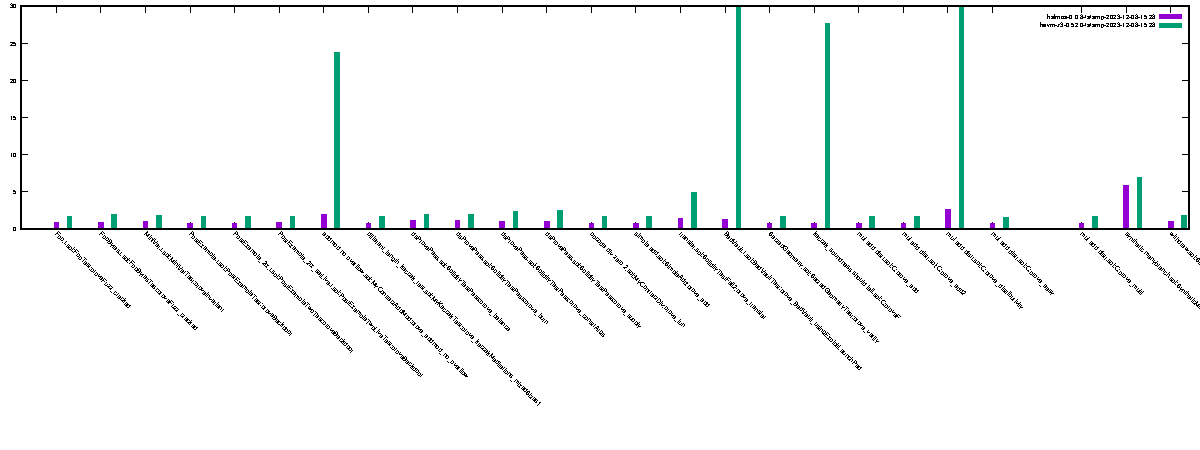
\includegraphics[scale=0.75]{boxchart}
%[1] \url{https://github.com/eth-sc-comp/benchmarks/}
%[2] \url{https://github.com/a16z/halmos}
%\end{frame}


%\begin{frame}[fragile=singleslide]{Contributing Back to hevm}
%
%The hevm repository uses \texttt{nix} for ease of development:
%
%
%
%You now have a full development environment, with all necessary tools installed, including Z3.
%\bigskip 
%
%hevm is written in Haskell, but there are many areas that can be contributed to without deep knowledge of Haskell. For example, expression simplification:
%
%\begin{Verbatim}[frame=single, framerule=0.2mm, framesep=2mm,fontsize=\footnotesize]
%    go (Add a b)
%      | b == (Lit 0) = a
%      | a == (Lit 0) = b
%      | otherwise = add a b
%\end{Verbatim}
%\end{frame}

% \section{Results}

% \begin{frame}[fragile=singleslide]{Results}

% We ran latest hevm, halmos, and kontrol (KEVM) on the Eth-SC Ethereum benchmarks [1], on an AMD 5950x with 5min timeout,  and 128GB of RAM. For more details: $\rightarrow$ see paper!
% {
% \begin{center}
% 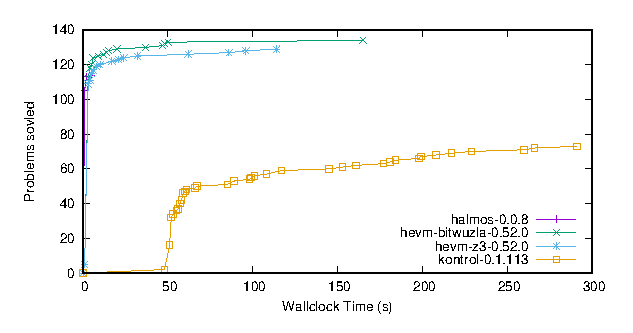
\includegraphics{cdf}
% \end{center}
% }


% [1] \qrcode[height=0.7cm]{https://github.com/eth-sc-comp/benchmarks/}\qquad  \url{https://github.com/eth-sc-comp/benchmarks/}
% \end{frame}


\section{Conclusions}

\begin{frame}[fragile=singleslide]{Limitations \& Future Work}
hevm has a number of inherent limitations:

\begin{itemize}
\item Loops are challenging. We have an iteration limit until which loops are examined
\item Recursion, and parametric calls can cause hevm to only partially explore the state
\item Complicated mathematical expressions (e.g. division, modulo) can cause a challenge
\item hevm is not verified, and neither are SMT solvers
\end{itemize}
\vspace{2ex}

Future work:
\begin{itemize}
\item Symbolic CopySlice handling -- I finally have an idea :)
\item Better handling of loops and recursion: include into IR, and solve for invariant via CHC
\end{itemize}

\bigskip

\quad  \qrcode[height=1cm]{https://github.com/ethereum/hevm/releases}
\qquad \url{https://github.com/ethereum/hevm/releases}

\end{frame}

%\section{Conclusions}
%\begin{frame}[fragile=singleslide]{Conclusions}
%
%hevm is a fully-featured, easy-to-use tool that can help find bugs in EVM bytecode. Its sophisticated IR is tailored to the EVM via Keccak- and array/map-specific rewrites to lower the complexity of solving the final SMT expression.
%\bigskip
%
%%Download hevm from \url{https://github.com/ethereum/hevm/releases}
%%\bigskip
%%\qrcode{https://github.com/ethereum/hevm/releases}
%
%Development environment:
%\begin{Verbatim}[frame=single, framerule=0.2mm, framesep=2mm,fontsize=\footnotesize]
%sh <(curl -L https://nixos.org/nix/install) --daemon
%git clone https://github.com/ethereum/hevm/
%nix-shell
%cabal repl test
%[...]
%> :main
%\end{Verbatim}
%
%\end{frame}



\end{document}
